\section{Results}
\label{sec:results}
In this section we'll look at the results we got from each of the different techniques outlined in \autoref{sec:methods}.

\paragraph{Execution notes.}
All the results were obtained by running our program with about 16 GB of working memory and 1 core per instance. The system running our program was equipped with an Intel Xeon \footnote{The cluster we worked on, is more thoroughly described here: \url{https://docs.dei.unipd.it/en/CLUSTER/Overview}}. The runtime for a sweep on the selected subsample rates is on the order of a few hours.

% \paragraph{Evaluation metrics.} In this work we focused on the Accuracy and F1 scores.


\subsection{Subsampling on the whole genome}
\begin{figure}[ht!]
    \centering
    \begin{subfigure}[t]{0.49\textwidth}
    \centering
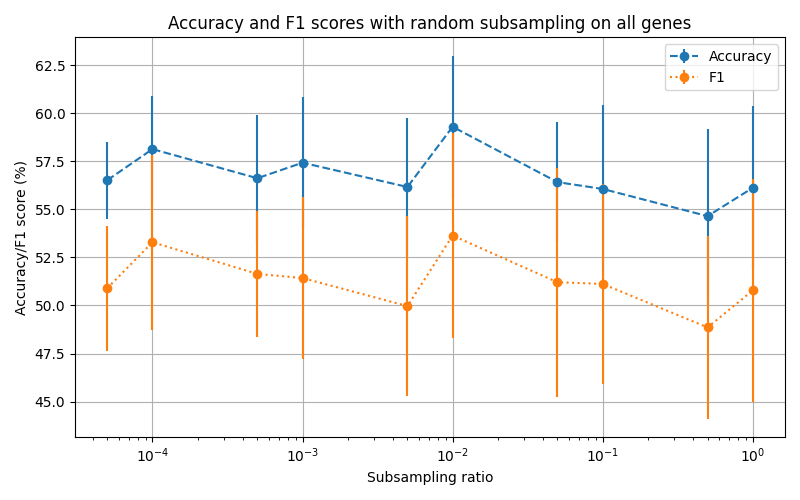
\includegraphics[width=\columnwidth]{figures/subsample_plot.png}
\caption{Plot of the scores when subsampling uniformly on the whole genome.}
\label{fig:res1a}
    \end{subfigure}
    \begin{subfigure}[t]{0.49\textwidth}
    \centering
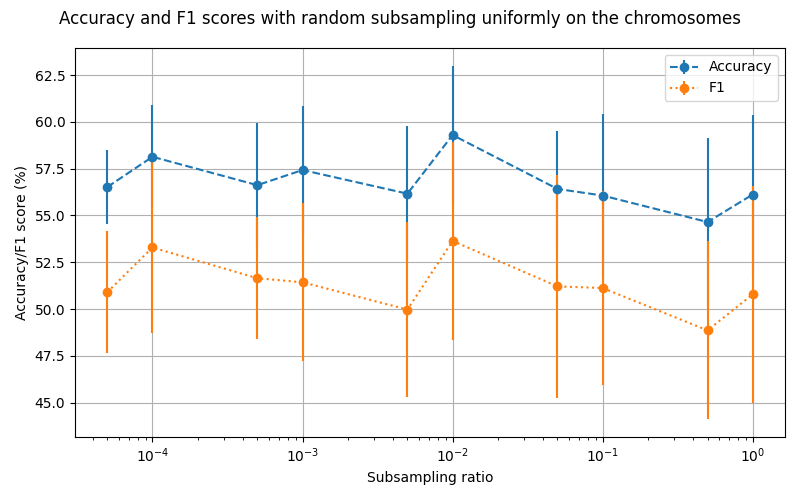
\includegraphics[width=\columnwidth]{figures/uniform_sample_low_ratio.png}
\caption{Plot of the scores when subsampling uniformly on each chromosome.}
\label{fig:res1b}
    \end{subfigure}
\caption{Plots of accuracy and F1 scores for different subsampling rates on the whole genome.}
\label{fig:res1}
\end{figure}

The first simple tests were done selecting a random subset of genes among all the SNPs that we had. The results for each subsampling rate are shown in \autoref{fig:res1}.
These plots show a mostly flat picture: both for the accuracy and F1 score there isn't a definite trend or variation as a function of the subsampling rate.

The only exception to this is \autoref{fig:res1a}, that shows a diminishing trend with the smallest subsampling rates. Nevertheless both of the last two data points are compatible with the middle points.

Remark that our experimental setup is designed to have no random components out of the subsampling step, thus no subsampling implies no randomization. For this reason the values for subsampling rate $1 = 10^0$ (no subsampling) are the same in the two plots of \autoref{fig:res1} and have no error bars.
This single values could be slightly far from than the true expected value because of random variation in the results. Thus the slight decrease between the "middle" subsampling rates and this last data point is probably not meaningful. 

\subsection{Annotated genes subsampling}
\begin{figure}[ht!]
\centering
\begin{subfigure}[ht]{\textwidth}
    \centering 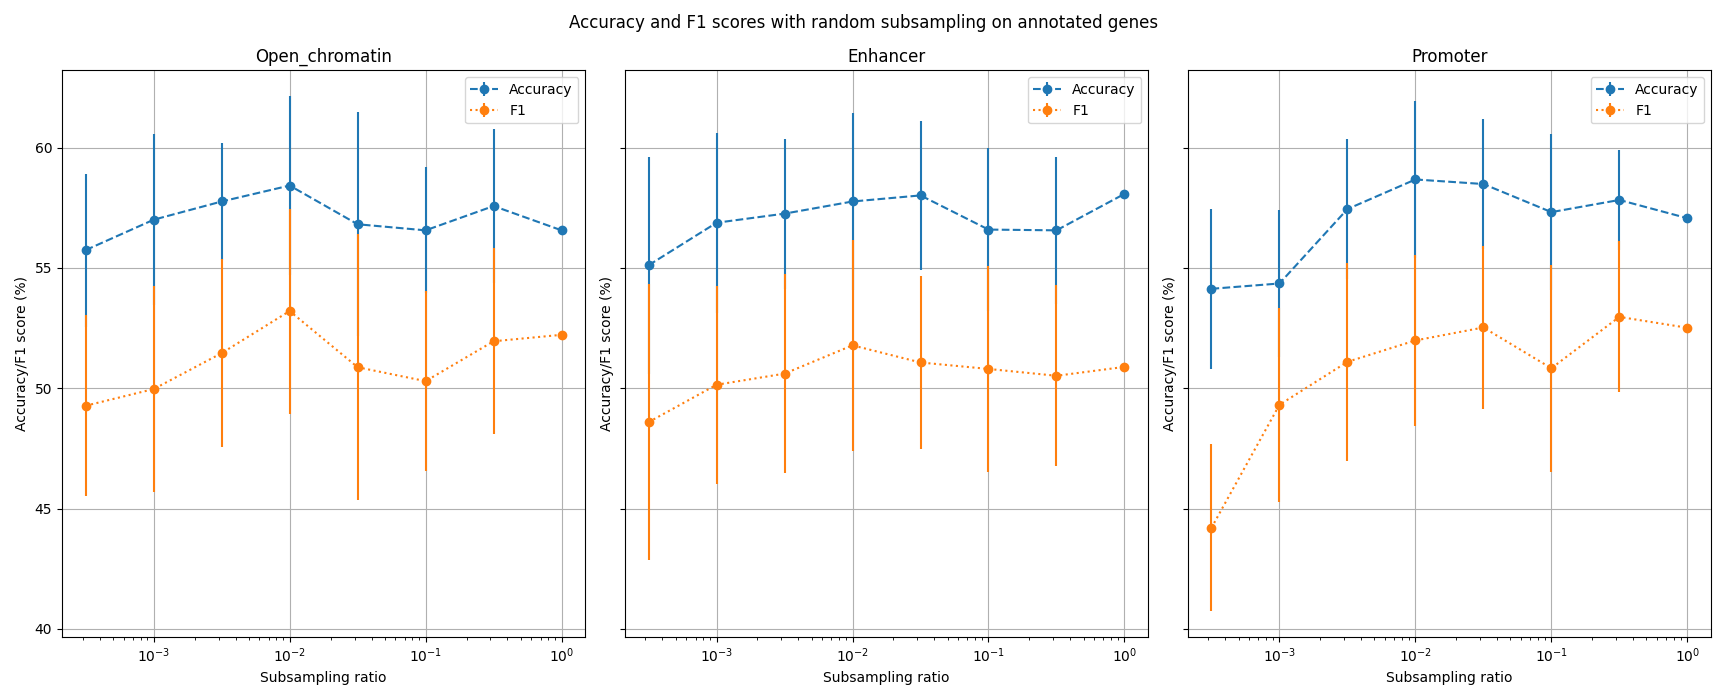
\includegraphics[width=\textwidth]{figures/subsample_annotated.png}
\caption{Plots of the scores while subsampling genes annotated in different categories.}
\label{fig:res2a}
\end{subfigure}

\begin{subfigure}[ht]{\textwidth}
\centering
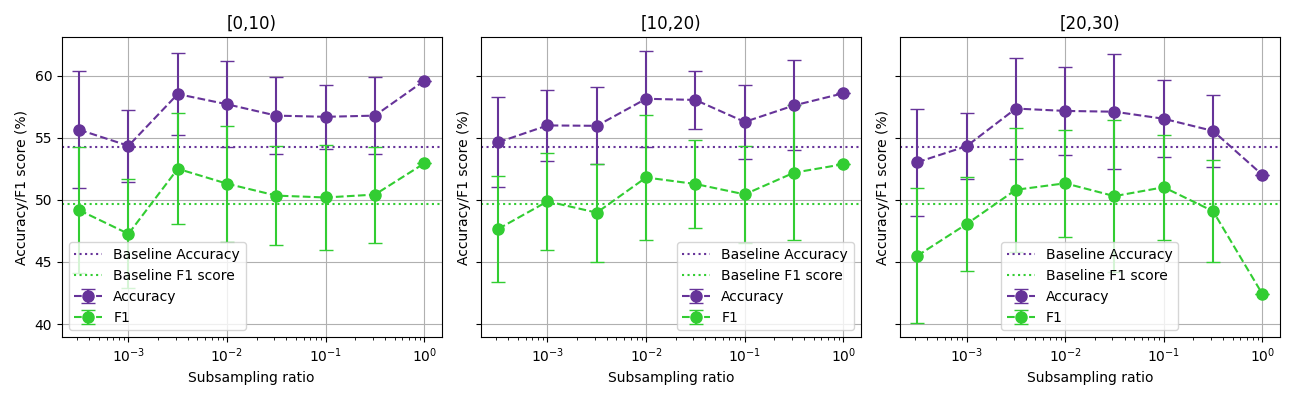
\includegraphics[width=\textwidth]{figures/subsample_ntissue.png}
\caption{Plots of the scores while using only genes with tissue number in a given range.}
\label{fig:res2b}
\end{subfigure}
\caption{Plots of the accuracy and F1 scores for the different subsampling rates on the annotated genes. Each single plot is done using only the genes annotated with the indicated values.}
\label{fig:res2}
\end{figure}

The second set of tests was done using only the annotated genes. The results on each set of similarly annotated genes are shown in \autoref{fig:res2}: \autoref{fig:res2a} shows the results using function annotations, and \autoref{fig:res2b} the results when selecting genes with tissue number in different intervals.

As before, these plots show a mostly flat picture, both for the accuracy and F1 score.


\subsection{Considerations on the results}
% Our results suck a lot.
Overall the results do not show any meaningful trend. The most likely pattern to be inferred from our data is a flat trend, meaning that the scores and subsampling rates are nearly independent. This seems to hold outside the extreme ends of our sampled interval of subsampling rates.

Another simple observation that can be drawn from our results is that keeping only a very small subset of genes (in the order of tens or less) has a negative effect on the scores.
This can be seen especially in the "Promoter" plot of \autoref{fig:res2a}, and could be a cause of the upwards trend on the left of \autoref{fig:res1a}.


